\chapter{LEN5 frontend}
\section{General block diagram}
\begin{figure}[hbt]
  \centering
  \makebox[\textwidth][c]{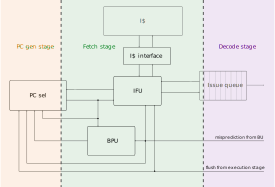
\includegraphics[width=1.2\textwidth]{img/frontend.pdf}}
  \caption{LEN5 frontend}
  \label{fig:frontend}
\end{figure}
Figure \ref{fig:frontend} shows a top-level block diagram of the LEN5 frontend, with the modules that were developed and that will be described in the following sections shown in solid black color. Gray blocks are instead the ones the frontend interfaces with.

The frontend is composed of two pipeline stages, name the \emph{\ac{PC} generation} and the \emph{fetch} stages. Figure \ref{fig:frontend} also shows the \emph{decode} stage, where the issue queue is found. This is basically a \acs{FIFO} that serves as a buffer interface between the frontend and the backend of the processor by storing a queue of instructions to be issue to the later stages of the pipeline.

In the \ac{PC} generation (\ac{PC} gen) stage the next \ac{PC} is selected among a number of different options by the \ac{PC} sel block, using a predefined priority and is then written on the output register of the stage. This register also serves as the pipeline register between the two stages, and that is why figure \ref{fig:frontend} shows a dashed gray line crossing the \ac{PC} sel block. The selection of the new \ac{PC} is carried out by a network of combinational logic, so that this stage always takes exactly one clock cycle.

In the fetch stage, the \ac{PC} is used by the \ac{IFU} to select and possibly read from memory the next instruction to be pushed to the issue queue. At the same time, the \ac{BPU} uses the current address to predict the next direction in case of branch and passes such information back to the \ac{PC} gen stage. Memory accesses are performed through the instruction cache interface which manages the control signals to the instruction cache. Regarding latency of the fetch stage, in a normal steady state the \ac{IFU} can provide one instruction each clock cycle to the issue queue, but in case of cache miss the number of cycles to resolve the stall can grow significantly, so the latency cannot be determined in advance. The issue queue is there exactly to provide some elasticity to the pipeline, by buffering already fetched instructions.

\subsection{Handshake signals}\label{sec:handshake}
The communication between each stage is always bidirectional, because in case of a stall caused for instance by a cache miss, by a full issue queue or by some other exceptional behavior down the pipeline, the \ac{PC} generation process must be interrupted along with the fetch. In order to do so, a handshake process handles the communication between each stage as well as between the instruction cache interface and the actual cache. This handshake mechanism is based on the {\smaller AXI} valid/ready protocol described below, even if it is not compliant with all the {\smaller AXI} specifications.

In each communication the source of data generates a \emph{valid} signal to indicate that the information is available, while the destination generates a \emph{ready} signal to indicate that it can accept such information \cite[p.~A3-41]{axi}. The handshake takes place and the information is successfully exchanged only at the rising clock edge when both valid and ready are asserted. For example, in figure \ref{fig:axi}, the handshake happens at the third rising edge of the clock.
\begin{figure}[hbt]
  \centering
  \includegraphics{img/axi.pdf}
  \caption{AXI handshake protocol}
  \label{fig:axi}
\end{figure}

When a source has information available (figure \ref{fig:axi_valid_ready}), it must assert valid and then wait until the corresponding ready is produced. It cannot wait for the ready before asserting valid.
\begin{figure}[hbt]
  \centering
  \subfloat[Valid before ready]{
    \label{fig:axi_valid_ready}
    \includegraphics{img/axi_valid_ready.pdf}} \\
  \subfloat[Ready before valid]{
    \label{fig:axi_ready_valid}
    \includegraphics{img/axi_ready_valid.pdf}}
  \caption{Possible handshake timings}
  \label{fig:axi_timings}
\end{figure}
On the other hand (figure \ref{fig:axi_ready_valid}), a destination is allowed to wait for its valid before asserting ready and it can also deassert ready before a corresponding valid arrives.

\section{\acs{PC} gen stage}
The selection of the next \ac{PC} is based on the following list of priorities, from highest to lowest:
\begin{enumerate}
  \item \textbf{Exception}: if an exception occurs, the \ac{PC} gen stage will receive the next starting address as the base address present in the vector table provided by the {\smaller CSR} unit.
  \item \textbf{Misprediction}: if a resolved branch is discovered to have been mispredicted, then the \ac{PC} gen stage resumes execution from the correct target if the branch was actually taken, or from the next sequential address from the branch \ac{PC} if it was actually not taken.
  \item \textbf{Branch prediction}: if the \ac{BPU} predicts a taken branch for the current \ac{PC} then it provides this stage with the predicted target address (see section \ref{}), which will be fetched at the next cycle, thus allowing for zero penalty branches when predicted correctly.
  \item \textbf{Default assignment}: if none of the conditions before occur, then the next \ac{PC} is selected as usual as the next sequential address, which corresponds to the current \ac{PC}+4 for word-aligned 32-bit instructions.
\end{enumerate}

\begin{figure}[hbt]
  \centering
  \makebox[\textwidth][c]{\includegraphics[width=1.2\textwidth]{img/pc_gen_stage.pdf}}
  \caption{\acs{PC} gen stage diagram}
  \label{fig:pc_gen_stage}
\end{figure}
Figure \ref{fig:pc_gen_stage} shows the diagram of this stage. This and all the following diagrams in this document are color coded so that input signals are in {\color{input_blue}{blue}}, output signals are in {\color{output_red}{red}}, internal signals in black and bit widths are in {\color{width_gray}{gray}}.

The heart of the \ac{PC} gen stage is the \texttt{pc\_priority\_enc} block, which is an encoder that takes as inputs all the status signals indicating a behavior different from the default and all the corresponding potential next \acp{PC}. In behavioral SystemVerilog (listing \ref{code:priorityenc}) it is described as a if-then-else chain, which gets synthesized as a list of cascading multiplexers implementing the desired priority\footnote{As opposed to the description using a case statement, which leads to a single parallel mux, with no priority encoded.}.
\begin{lstlisting}[
  language=Verilog,
  caption={\texttt{pc\_priority\_enc} description},
  captionpos=b,
  label=code:priorityenc
]
  always_comb begin: pc_priority_enc
    if (except_i) begin
      next_pc = except_pc_i;
    end else if (res_valid_i && res_mispredict_i) begin
      if (res_taken_i) begin
        next_pc = res_target_i;
      end else begin
        next_pc = adder_out;
      end
    end else if (pred_taken_i) begin
      next_pc = pred_target_i;
    end else begin
      next_pc = adder_out;
    end
  end: pc_priority_enc
\end{lstlisting}

In order to save resources, a single adder is used to generate both the next sequential address and the next \ac{PC} after a mispredicted not taken branch. A multiplexer driven by the misprediction signals is used to select the right operand.

The final selected next \ac{PC} is fed into the \texttt{pc\_reg} output register for the later stages. The enable of this register is controlled by the signal \texttt{fetch\_ready\_i} which comes from the fetch stage and disables the \ac{PC} generation if a stall occurs. This is part of the handshake mechanism described in section \ref{sec:handshake}, even if there is no \emph{valid} signal from the \ac{PC} gen stage, as it is redundant due to the fact that a valid new \ac{PC} is always present at the output register.

\section{Instruction cache interface}
\begin{figure}[hbt]
  \centering
  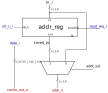
\includegraphics{img/icache_ifc.pdf}
  \caption{Instruction cache interface}
  \label{fig:icache_ifc}
\end{figure}
The instruction cache interface (figure \ref{fig:icache_ifc}) is responsible for translating the fetch requests coming from the \ac{IFU} into compliant valid/ready handshake signals for both address and data to the instruction cache. This unit basically provides two main benefits. First, it simplifies the control of the \ac{IFU}, by delegating the handshake process. Second, and more important, it provides an additional separation layer between the core frontend and the instruction cache with modularity in mind so that, should the cache block be modified, only this interface block needs to be updated, while the signals coming from the \ac{IFU} module would remain unchanged.

\subsection{Control \acs{FSM} and timing}
While the data signals are as straightforward as simple wires connecting \texttt{pc\_i} and \texttt{cache\_out\_o} with \texttt{addr\_o} and \texttt{data\_i} respectively, the core of this interface lies in its control unit.
\begin{figure}[hbt]
  \centering
  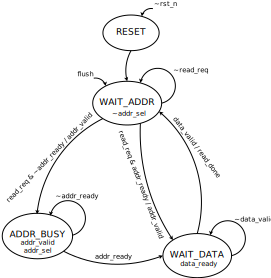
\includegraphics[scale=.8]{img/icache_ifc_fsm.pdf}
  \caption{Instruction cache interface \acs{FSM}}
  \label{fig:icache_ifc_fsm}
\end{figure}
It is a simple Mealy \acs{FSM} (figure \ref{fig:icache_ifc_fsm}) that after reset waits for a read request from the \ac{IFU}, then checks if the instruction cache is ready to receive an address and finally waits for a valid cache line to be read.

\begin{figure}[hbt]
  \centering
  \includegraphics{img/cache01.pdf}
  \caption{Normal cache read}
  \label{fig:cache01}
\end{figure}
Figure \ref{fig:cache01} shows a normal cache read, where the instruction cache is immediately ready to receive an address which hits and produces the requested data at the next clock cycle. From this timing diagram it is also clear why a Mealy \acs{FSM} is needed: the signal \texttt{addr\_valid} needs to be asserted combinationally in the same clock cycle in which \texttt{read\_req} arrives, so that the address handshake can take place immediately. Otherwise, with a Moore machine, one clock cycle would be wasted at each request, rendering impossible to sustain one instruction per clock cycle fetch. Another possibility would have been not to include such signal as a Mealy output of the machine and instead connect it with a wire outside the \acs{FSM}, which would lead to the same exact result, but was deemed as less readable.

\begin{figure}[hbt]
  \centering
  \includegraphics[width=\textwidth]{img/cache02.pdf}
  \caption{Cache not ready on address}
  \label{fig:cache02}
\end{figure}
Figure \ref{fig:cache02} shows another possibility when the instruction cache is not ready to receive an address at the time when a request arrives. In this case the \acs{FSM} waits until the cache become ready in the \texttt{ADDR\_BUSY} state. The state machine could just as well wait in the \texttt{WAIT\_ADDR} state, but the additional state was introduced for robustness with \texttt{addr\_valid} as a Moore output, so that this way there is no need for the \texttt{read\_req} signal to stay active until the cache is ready. This is another point in favor of a Mealy \acs{FSM} instead of the connection of combinational outputs externally.

\begin{figure}[hbt]
  \centering
  \includegraphics[width=\textwidth]{img/cache03.pdf}
  \caption{Cache miss}
  \label{fig:cache03}
\end{figure}
Finally, figure \ref{fig:cache03} shows the case of a cache miss, in which the \ac{FSM} waits while keeping \texttt{data\_ready} asserted. This state could potentially last for many clock cycles.

\section{\acf{IFU}}
\begin{figure}[hbt]
  \centering
  \makebox[\textwidth][c]{\includegraphics[width=1.2\textwidth]{img/fetch_stage.pdf}}
  \caption{Fetch stage diagram}
  \label{fig:fetch_stage}
\end{figure}

\section{\acf{BPU}}

\section{Branch unit}